\documentclass[12pt,a4paper]{article}
\usepackage[utf8]{inputenc}
\usepackage{amsmath}
\usepackage{textcomp}

\usepackage{geometry}
\geometry{a4paper,left=25mm,right=25mm, top=2cm, bottom=2cm} 

\usepackage{verbatim}

 \usepackage{mathptmx}
 \usepackage[scaled=.90]{helvet}
 \usepackage{courier}

\usepackage[utf8]{inputenc}

\usepackage{listings}
\usepackage{color}

\usepackage{graphicx}
 
\definecolor{dkgreen}{rgb}{0,0.6,0}
\definecolor{gray}{rgb}{0.5,0.5,0.5}
\definecolor{mauve}{rgb}{0.58,0,0.82}

\pagestyle{empty}
\lstset{numbers=left,language=C++}
\lstset{showstringspaces=false,
basicstyle=\ttfamily\footnotesize,
breaklines=true,
tabsize=3,
commentstyle=\color{dkgreen},       % comment style
}

%keine einrückungen bei absatz
\parindent 0pt

\begin{document}
\title{Übung 7}
\author{Bernhard Selymes, Reinhard Penn}
\date{Jänner 2012}

\normalsize

%Pfad zu c++ Dateien
\newcommand{\CodePath}{../CarRental/CarRental/}

%Beginn des Dokuments
\section{Organisatorisches}

\subsection{Team}
	\begin {itemize} 
		\item Reinhard Penn, s1110306019 
		\item Bernhard Selymes, s1110306024
	\end {itemize}

\subsection{Aufteilung}
	\begin {itemize} 
		\item Reinhard Penn
			\begin {itemize}
				\item Planung
				\item Klassendiagramm
				\item Implementierung der Klassen CarRental, ConcreteCar und Unterklassen
				\item Testen aller Klassen
			\end {itemize}
		\item Bernhard Selymes
			\begin {itemize}
				\item Planung
				\item Klassendiagramm
				\item Implementierung der Klassen ICar, Decorator und Unterklassen
				\item Dokumentation		
			\end {itemize}
	\end {itemize}


\subsection{Zeitaufwand}
	\begin {itemize}
		\item geschätzte Mh: 12
		\item tatsächlich: Reinhard (5h), Bernhard  (6h)
	\end {itemize}


\section{Systemspezifikation}
Eine Sofware für die Verwaltung von Kraftfahrzeuge in einer Autovermietung soll entworfen werden. Die Kraftfahrzeuge gehören zu einer Klasse, die den Preis des Fahrzeugs bestimmt. Ein Kraftfahrzeug kann zusätzlich Sonderausstattungen haben, die zusätzlich etwas kosten.
\\


\newpage
\section {Systementwurf}

\subsection {Klassendiagramm}

%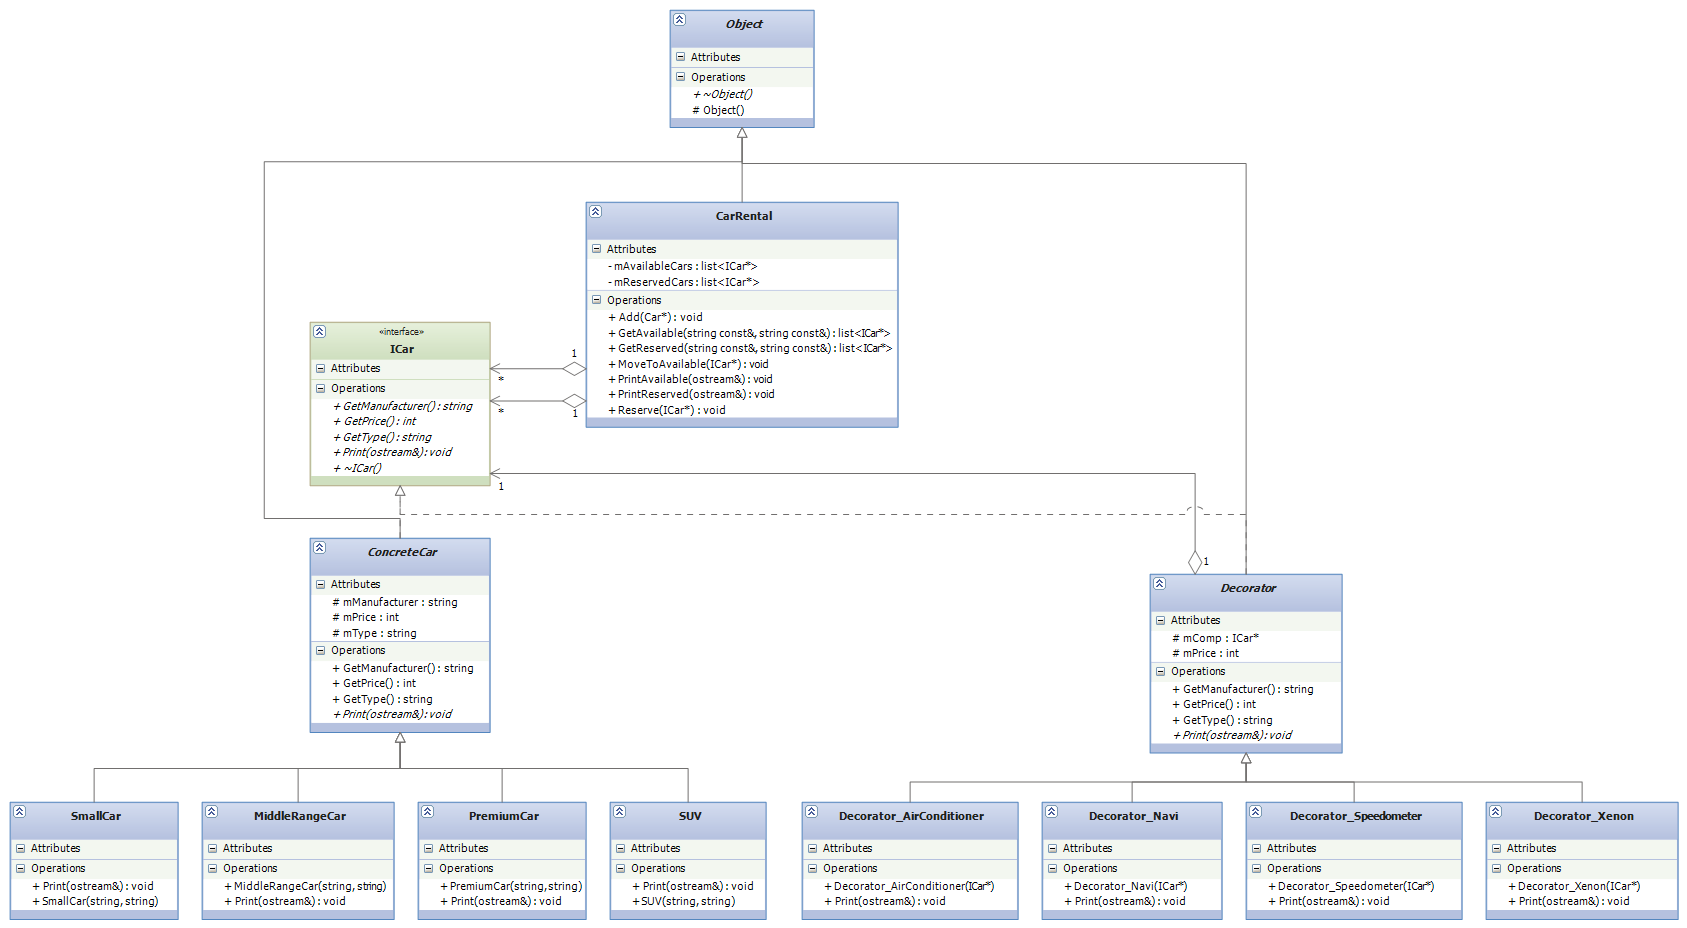
\includegraphics[angle=90,scale=0.5] {../Klassendiagramm.png}

\newpage
\subsection {Komponentenübersicht}
\begin {itemize} 
	\item Klasse "Object":
	\newline
	Basis aller Basisklassen.
	
	\item Interface "ICar":
	\newline
	Schnittstellen der Funktionen.

	\item Klasse "ConcreteCar":
	\newline
	Basisklasse für die einzelnen konkreten Kraftfahrzeuge.

	\item Klassen "SmallCar, MiddleRangeCar, PremiumCar und SUV":
	\newline
	Konkrete Klassen von Kraftfahrzeugen.

	\item Klasse "Decorator":
	\newline
	Basisklasse für die konkreten Sonderausstattungen.
	
	\item Klassen "AirConditioner, Navi, Speedometer und Xenon":
	\newline
	Konkrete Sonderausstattungen.

	\item Klasse "CarRental":
	\newline
	Verwaltet die Kraftfahrzeuge.
			
\end {itemize}

\newpage
\section {Komponentenentwurf}
\subsection {Klasse "Object"}
Abstrakte Basisklasse aller Klassen. Von ihr werden alle anderen Klassen abgeleitet. Beinhaltet einen virtuellen Destruktor.

\subsection {Interface "ICar"}
Definiert die Schnittstellen der Methoden. Hat einen virtuellen Destruktor.
\\

\subsection {Klasse "ConcreteCar"}
Basisklasse für die konkreten Kraftfahrzeuge. Hat protected Member die den Hersteller, den Preis und den Typ speichern. Hat drei Get-Methoden für diese member. Hat eine abstrakte Methode "Print" die in den Unterklassen implementiert wird.
\\

\subsection {Klassen "SmallCar, MiddleRangeCar, PremiumCar und SUV"}
Konkrete Klassen von Kraftfahrzeugen.
\\

\textbf {Methode "Print": } 
\newline
Schnittstelle:
\newline
Parameter: ostream\&
\newline
Rückgabetyp: void
\newline
Wird je nach Klassen entsprechend implementiert. Gibt aus um welche Klasse es sich handelt und danach die entsprechenden Daten des Fahrzeugs.
\\

\subsection {Klasse "Decorator"}
Hat einen Member der den Preis speichert und einen der einen Pointer auf das Objekt, das er dekoriert, speichert. Die Funktion "Print" ist abstrakt. Hat drei Get-Methoden, die bis ganz in die Tiefe gehen (bis zum Kraftfahrzeug) und dann den Wert von dort zurückliefern. Beim Preis werden die Werte aufaddiert.
\\

\subsection {Klassen "AirConditioner, Navi, Speedometer und Xenon"}
Konkrete Ausstattungen.
\\

\textbf {Konstruktoren: } 
\newline
Schnittstelle: 
\newline
Parameter: ICar*
\newline
Überprüft den übergebenen Parameter auf Gültigkeit und weist den konkreten Preis zu.
\\

\textbf {Methode "Print": } 
\newline
Schnittstelle:
\newline
Parameter: ostream\&
\newline
Rückgabetyp: void
\newline
Ruft die Printfunktion des Objektes, das es dekoriert, auf und gibt dann aus um welche Sonderausstattung es sich handelt und den Preis davon.
\\

\subsection {Klasse "CarRental"}
Enthält eine Liste mit verfügbaren Kraftfahrzeugen und eine mit reservierten. Hat Get-Methoden für diese. Hat Methoden zum hinzufügen und verschieben zwischen den zwei Listen.
\\

\textbf {Methoden "PrintAvailable" und "PrintReserved": } 
\newline
Schnittstelle:
\newline
Parameter: ostream\&
\newline
Rückgabetyp: void
\newline
Gibt die Daten (Hersteller, Typ, Preis vom Fahrzeug, Sonderausstattungen und Preis davon und Gesamtpreis (Fahrzeug mit Ausstattungen)) aus.
\\

\textbf {Methoden "GetAvailable" und "GetReserved": } 
\newline
Schnittstelle:
\newline
Parameter: string const\&, string const \&
\newline
Rückgabetyp: list mit ICar*
\newline
Geben eine Liste zurück in der die Kraftfahrzeuge enthalten sind die der angegebenen Herstellermarke und Typ des Fahrzeugs entsprechen.
\\

\newpage
\section {Source Code}

\lstinputlisting[language=C++]{\CodePath Object.h}
\lstinputlisting[language=C++]{\CodePath Object.cpp}
\newpage

\lstinputlisting[language=C++]{\CodePath ICar.h}
\newpage

\lstinputlisting[language=C++]{\CodePath ConcreteCar.h}
\newpage
\lstinputlisting[language=C++]{\CodePath ConcreteCar.cpp}
\newpage

\lstinputlisting[language=C++]{\CodePath SmallCar.h}
\newpage
\lstinputlisting[language=C++]{\CodePath SmallCar.cpp}
\newpage

\lstinputlisting[language=C++]{\CodePath MiddleRangeCar.h}
\newpage
\lstinputlisting[language=C++]{\CodePath MiddleRangeCar.cpp}
\newpage

\lstinputlisting[language=C++]{\CodePath PremiumCar.h}
\newpage
\lstinputlisting[language=C++]{\CodePath PremiumCar.cpp}
\newpage

\lstinputlisting[language=C++]{\CodePath SUV.h}
\newpage
\lstinputlisting[language=C++]{\CodePath SUV.cpp}
\newpage

\lstinputlisting[language=C++]{\CodePath Decorator.h}
\newpage
\lstinputlisting[language=C++]{\CodePath Decorator.cpp}
\newpage

\lstinputlisting[language=C++]{\CodePath Decorator_AirConditioner.h}
\newpage
\lstinputlisting[language=C++]{\CodePath Decorator_AirConditioner.cpp}
\newpage

\lstinputlisting[language=C++]{\CodePath Decorator_Navi.h}
\newpage
\lstinputlisting[language=C++]{\CodePath Decorator_Navi.cpp}
\newpage

\lstinputlisting[language=C++]{\CodePath Decorator_Speedometer.h}
\newpage
\lstinputlisting[language=C++]{\CodePath Decorator_Speedometer.cpp}
\newpage

\lstinputlisting[language=C++]{\CodePath Decorator_Xenion.h}
\newpage
\lstinputlisting[language=C++]{\CodePath Decorator_Xenion.cpp}
\newpage

\lstinputlisting[language=C++]{\CodePath CarRental.h}
\newpage
\lstinputlisting[language=C++]{\CodePath CarRental.cpp}
\newpage

\lstinputlisting[language=C++]{\CodePath Main.cpp}
\newpage

\section {Testausgaben} 

\begin {verbatim}

\end {verbatim}


\end{document}